\documentclass[conference]{IEEEtran}
\IEEEoverridecommandlockouts
% The preceding line is only needed to identify funding in the first footnote. If that is unneeded, please comment it out.
\DeclareRobustCommand{\IEEEauthorrefmark}[1]{\smash{\textsuperscript{\footnotesize #1}}}
\usepackage{cite}
\usepackage{amsmath,amssymb,amsfonts}
\usepackage{algorithmic}
\usepackage{graphicx}
\usepackage{textcomp}
\usepackage{xcolor}
\usepackage{multicol}
\usepackage{algorithmic}
\usepackage{hyperref}

\def\BibTeX{{\rm B\kern-.05em{\sc i\kern-.025em b}\kern-.08em
    T\kern-.1667em\lower.7ex\hbox{E}\kern-.125emX}}
\begin{document}

\title{Acquisition Time in Dual Shunt-Based Current Sensing for PMSM FOC}

\author{
    \IEEEauthorblockN{
        Mark Wendler\IEEEauthorrefmark{1}, 
        and József Kopják\IEEEauthorrefmark{2} 
    }

    \IEEEauthorblockA{
        \IEEEauthorrefmark{1} Doctoral School of Applied Informatics and Applied Mathematics, 
        Óbuda University, Budapest, Hungary \\
        Email: mark.wendler@phd.uni-obuda.hu
    }

    \IEEEauthorblockA{
        \IEEEauthorrefmark{2} Kandó Kálmán Faculty of Electrical Engineering, 
        Óbuda University, 
        Budapest, Hungary \\
        Email: kopjak.jozsef@kvk.uni-obuda.hu
    }

}


\maketitle

\begin{abstract}
High-efficiency field‑oriented control (FOC) of permanent-magnet synchronous motors (PMSM) hinges on precise, low-latency stator current measurement synchronized to PWM. In sensorless drives, current‑measurement error propagates through the position estimator and can degrade efficiency compared to sensored FOC. This article translates estimator accuracy targets into concrete ADC and PWM requirements, with a practical focus on shunt topologies. We show why acquisition time (settling + sample-and-hold time) is usually more critical than nominal analog-to-digital converter (ADC) bandwidth, how modulation index and space-vector modulation (SVM) windows constrain sampling, and how topology choices affect both precision and timing.
\end{abstract}



\begin{IEEEkeywords}
Embedded Systems, Motor Control, PMSM, Current sensing, Dual shunt
\end{IEEEkeywords}

\section{Overview and Scope}
\label{sec:overview}
Field-oriented control (FOC) of permanent-magnet synchronous motors (PMSMs) relies on precise, low-latency phase-current measurements that are time-aligned to the pulse-width modulation (PWM) waveform \cite{Krause2013,Krishnan2010}. While many analyses treat current measurement as ideal, practical inverter and signal-chain constraints (deadtime, switching transients, amplifier settling, ADC acquisition windows) make the \emph{timing of acquisition} as important as nominal ADC resolution \cite{Bose2002,Kester2005}. This paper focuses on shunt-based current sensing and shows how current-measurement precision—especially in \emph{sensorless} operation—drives position-estimator accuracy, efficiency performance \cite{ACTAjaffer_omer_ghareeb_dynamic_2025,Holtz2002, ACTAjneid_integrated_2024}.


\subsection{Topologies considered}
We review and compare four shunt topologies that dominate cost- and size-constrained drives visualised on figure \ref{fig:currentSensing}:
\begin{enumerate}
  \item \textbf{In-line phase shunts} (one per phase at the motor terminals): highest accuracy and simplest reconstruction. Requires isolation at higher bus voltages and careful handling of common-mode transients \cite{Bose2002}.
  \item \textbf{Low-side three-shunt} (one shunt per phase return): high accuracy with reduced common-mode stress \cite{Krause2013}.
  \item \textbf{Low-side two-shunt}: similar to three-shunt but lower bill of materials. The 3 shunt can be reconstructed still relatively simple with Kirchhoff's Current Law.  $i_a{+}i_b{+}i_c{=}0$ \cite{Kester2005}.
  \item \textbf{Low-side single-shunt} (DC return): most economical and compact, but requires current reconstruction and imposes the tightest sampling-window constraints at certain modulation indexes and sector boundaries \cite{Bose2002,VanDerBroeck1986}.
\end{enumerate}
\begin{figure}
    \centering
    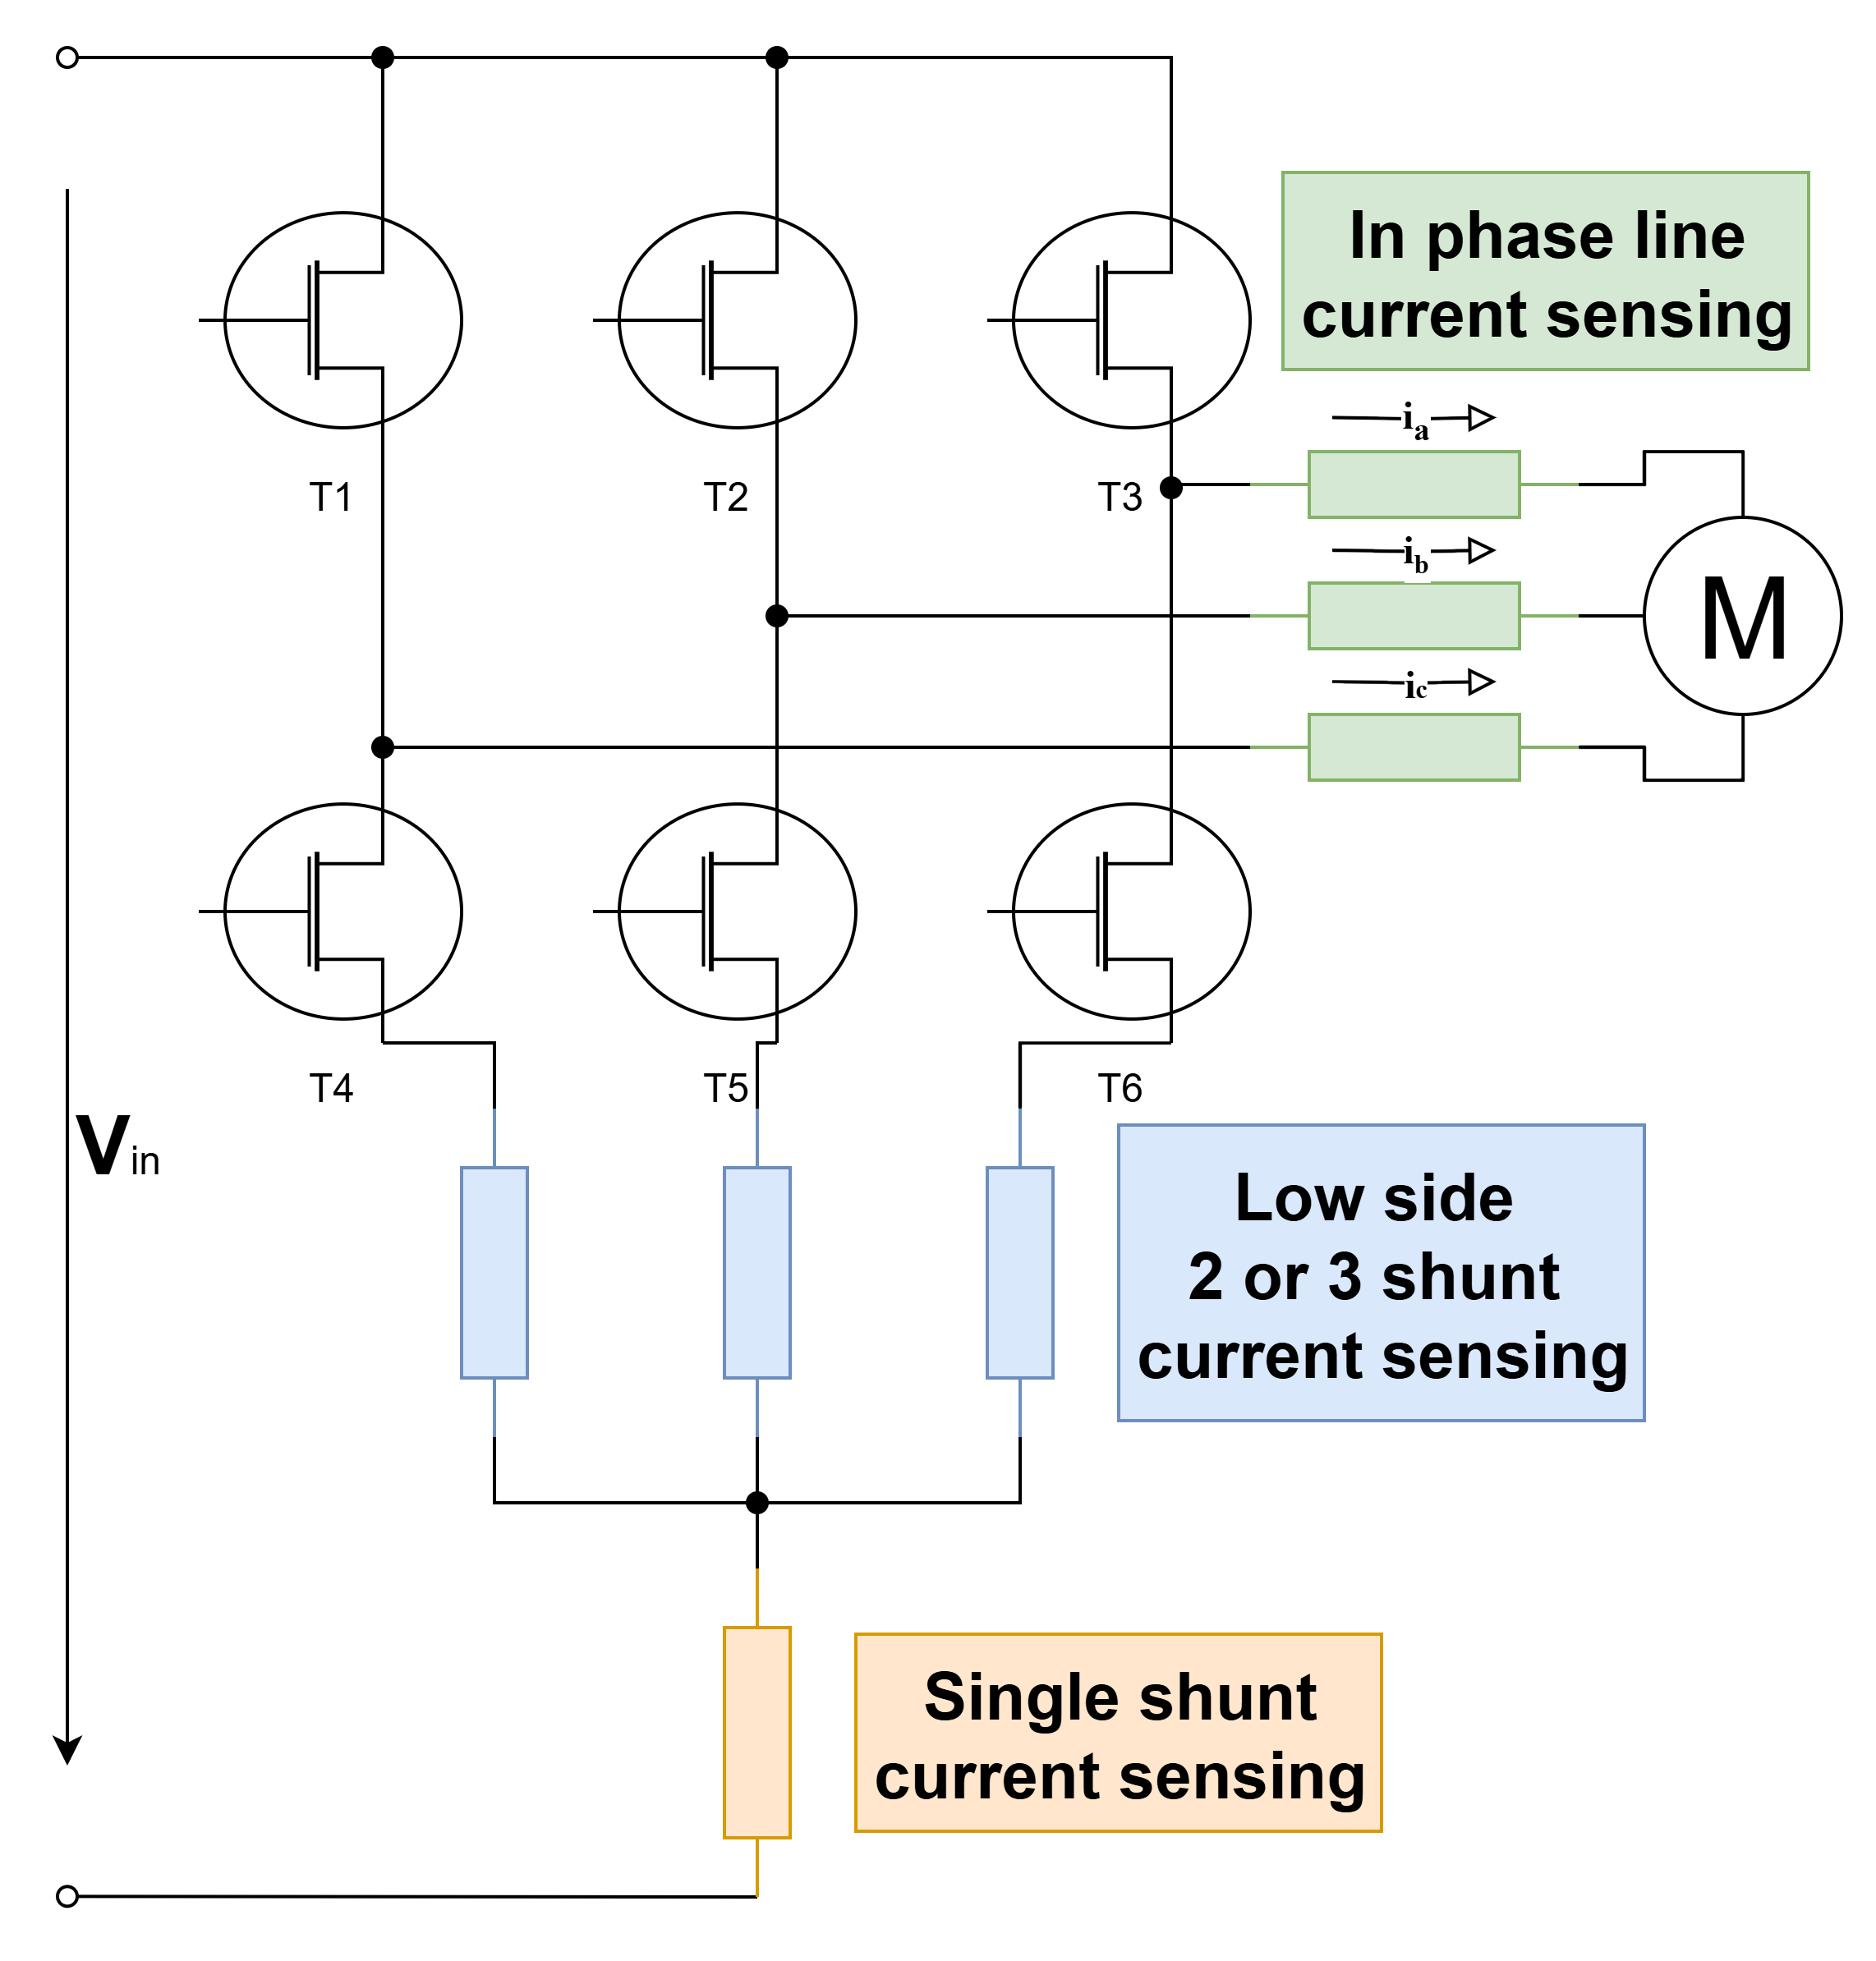
\includegraphics[width=1\linewidth]{Drawings/CurrentMeasWithCurrentLabel.png}
    \caption{3-phase Current sensing topologies}
    \label{fig:currentSensing}
\end{figure}

\subsection{Control, PWM, and timing preconditions}
\label{subsec:pwm-assumptions}

 We take as a \emph{hard requirement} that the analog sample is fully acquired and settled \emph{within} the valid PWM sampling window. If we don’t wait for the acquisition time, the ADC’s sample-and-hold latches a still-settling (wrong) value and introduce a hardly predictable value. \cite{wendler_enhancing_2025}

In this article, further assumptions and scenarios are used to keep the equations clear.
\begin{itemize}
    \item center-aligned PWM with space-vector modulation (linear SVM, split zero vectors);
    \item  ADC sampling is triggered at the center of active-vector plateaus;
    \item no clamped SVM and no enforced minimum on-time unless stated otherwise;
    \item deadtime, gate-driver propagation delay, and switching transient decay are captured in $t_{\mathrm{blank}}$;
    \item trigger jitter and timer/ADC dispersion are captured in $t_{\mathrm{margin}}$;
    \item $T_{sw}=1/f_{sw}$ denotes the full PWM period (carrier period).
\end{itemize}

\begin{equation}
  t_{\mathrm{acq}} \;\le\; t_{\mathrm{win}}
  \qquad\text{with}\qquad
  t_{\mathrm{win}} \;=\; t_{\mathrm{on}} \;-\; t_{\mathrm{blank}} \;-\; t_{\mathrm{margin}}
  \label{eq:precondition}
\end{equation}
\noindent \emph{Meaning of terms:}
\begin{itemize}
  \item $t_{\mathrm{acq}}$ — \textbf{acquisition/settling time}: the analog time needed for the shunt\,$\rightarrow$\,PGA/op-amp\,$\rightarrow$\,ADC input (and sample/hold) to settle to the target error band.
  \item $t_{\mathrm{win}}$ — \textbf{valid sampling window}: the portion of the SVM segment where switching transients are sufficiently decayed to allow accurate sampling.
  \item $t_{\mathrm{on}}$ — \textbf{active-vector on-time} for the relevant SVM segment (sets the geometric “ceiling” of the window).
  \item $t_{\mathrm{blank}}$ — \textbf{blanking time} after edges (deadtime + edge ringing / common-mode feedthrough and any enforced hardware blanking).
  \item $t_{\mathrm{margin}}$ — \textbf{guard time} for clock jitter, trigger dispersion.
\end{itemize}

\begin{figure}
    \centering
    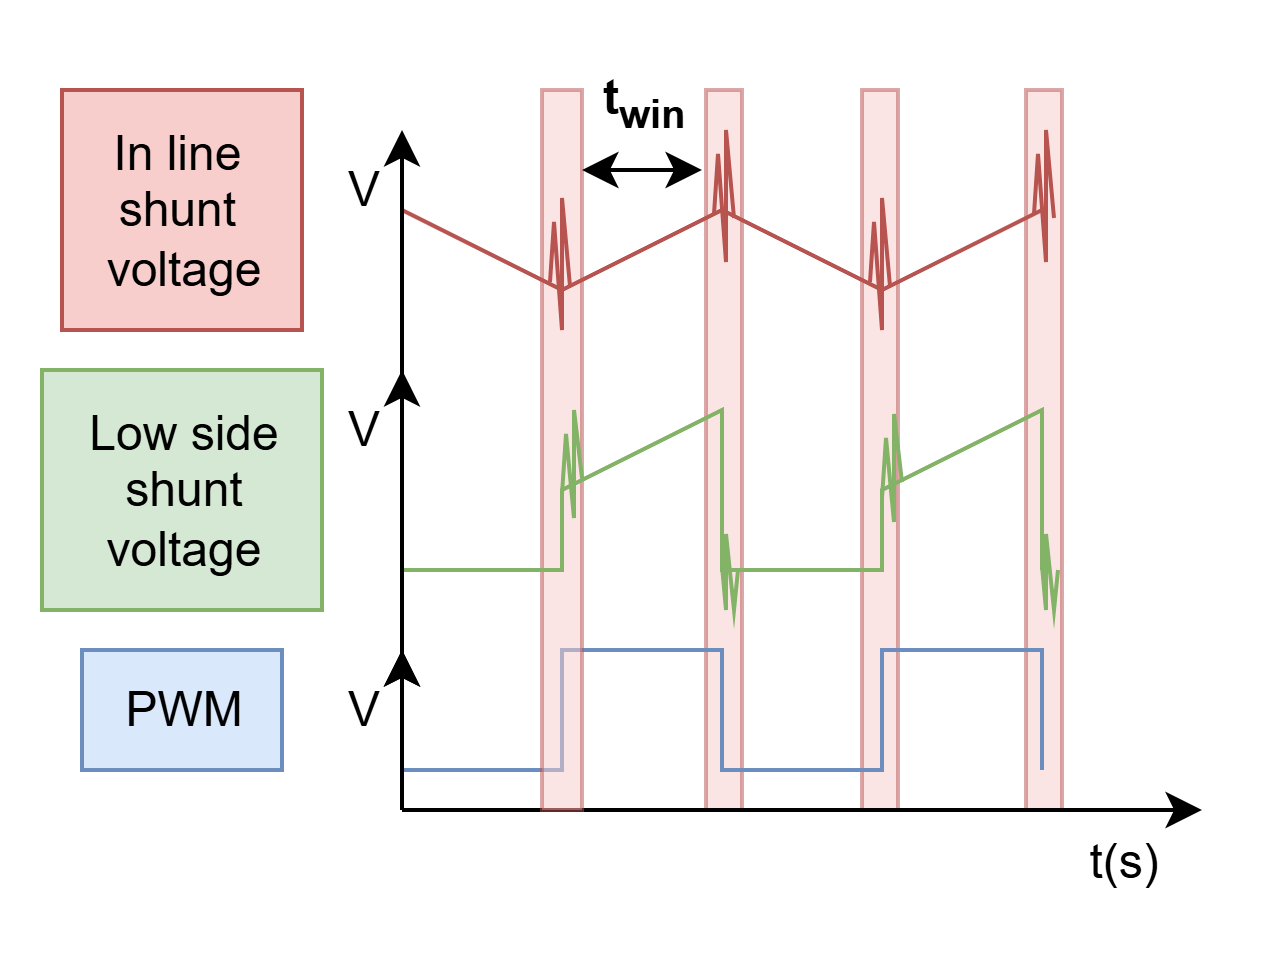
\includegraphics[width=1\linewidth]{Drawings/SwitchingNoise.png}
    \caption{Sampling window}
    \label{fig:samplingWin}
\end{figure}

\medskip
The \eqref{eq:precondition} is a \emph{physical constraint} for FOC accuracy. By contrast, many works emphasize the ADC “throughput” interval \(t_{\mathrm{acq}}{+}t_{\mathrm{conv}}\) or headline mega sample per second (MSPS) and treat it as the primary selection metric; however, once the sample is captured and held \emph{inside} $t_{\mathrm{win}}$, the conversion time \(t_{\mathrm{conv}}\) may complete later (even in the next half-period) without degrading the instantaneous measurement fidelity \cite{Kester2005,Bose2002}. Consequently, MSPS is not a reliable technical metric for direct evaluation, unless equation \eqref{eq:precondition} is satisfied. See representative throughput-centric treatments in \cite{ADI_EE365_2013,NXP_AN4608_2012,MathWorks_MCB_Sampling_2025,TI_SLAAE96A_2023,ST_AN3116_2010,Microchip_AN1078_2010}.

\medskip
For dual and triple shunt measurements we assume space-vector modulation (SVM) with center-aligned PWM, and schedule ADC triggers at the \emph{centers of active vectors} to minimize switching transients \cite{VanDerBroeck1986,Bose2002}. The blanking term \(t_{\mathrm{blank}}\) includes dead-time and edge-ringing/CM feedthrough; \(t_{\mathrm{margin}}\) covers clock jitter and trigger dispersion.

\medskip
ADC throughput \((t_{\mathrm{acq}}{+}t_{\mathrm{conv}})^{-1}\) still matters for picking the \emph{loop update rate} (single or double update per carrier), DMA bandwidth, and multi-channel interleaving, but it is \emph{secondary} to \eqref{eq:precondition} for measurement accuracy. Meeting \eqref{eq:precondition} enables deterministic, center-of-vector sampling, after which conversion may pipeline into the next half-period without penalty \cite{wendler_analysis_2025,kofler_sensorless_2025}. 

\subsection{Precision challenge and why acquisition time matters}
In sensorless FOC, the position estimator maps current error to electrical angle error; small increases in current-measurement noise/offset directly increase torque ripple and copper loss, particularly at low speed/weak back-EMF \cite{wendler_mechanical_2024}. Achieving the required \emph{system} Effective number of bits (ENOB) at the control update rate therefore hinges on capturing a clean sample \emph{inside} $t_{\text{win}}$. Headline ADC bandwidth or “MSPS” figures are insufficient if the input network cannot settle within the available window \cite{wendler_enhancing_2025}. Throughout the paper we emphasize specifying and validating \emph{acquisition/settling time} rather than generic bandwidth.

\subsection{Modulation index definition (for clarity)}

To avoid ambiguity, we define the SVM modulation index as

\begin{equation}
  m \;=\; \frac{V_{\text{ref}}}{V_{\text{dc}}/\sqrt{3}} \,,
  \label{eq:modindex}
\end{equation}

so that $m{=}1$ corresponds to the linear SVM limit \cite{VanDerBroeck1986,Bose2002}. Alternative definitions exist (e.g., based on line-to-line peak). There are other modulation index definitions easy to mix.
Discussions of single-shunt blind spots, minimum on-time, and clamped SVM strategies in this article assume \eqref{eq:modindex}.

\subsection{Performance metrics used in this paper}

We evaluate topologies using:
\begin{itemize}
  \item \textbf{System ENOB at loop bandwidth} (includes sensor, PGA, ADC) \cite{Kester2005}.
  \item \textbf{Acquisition/settling time} to a specified error band (e.g., $\pm\frac{1}{2}$\,LSB or ppm target) under realistic common-mode steps \cite{Kester2005}.
 % \item \textbf{Aperture jitter} {$\sigma_t$} mapped to current error $\sigma_{I,\text{jitt}}\!\approx |di/dt|\,\sigma_t$, with $di/dt \!\approx V/L$ \cite{Kester2005}.
  
  \item \textbf{Window robustness} vs.\ modulation index $m$ (presence/absence of blind spots; need for clamped SVM or minimum on-time) \cite{VanDerBroeck1986,Bose2002}.

\end{itemize}


\section{From Current Precision to Sensorless Estimator Accuracy and Efficiency}
\label{sec:precision-estimator}

In sensorless FOC, the rotor electrical angle \({\theta}_e\) is inferred from the applied voltages and measured currents through an observer or phase-locked loop (PLL) based on the PMSM model \cite{Vas1998,Holtz2002,Krishnan2010}. Any error in the measured phase currents \(\{i_a,i_b,i_c\}\) propagates to the \(dq\) currents, back-EMF estimates, and ultimately to the angle estimate.

\subsection{Measurement error taxonomy}
We decompose the instantaneous current error (referred to the ADC input after gain) as
\begin{equation}
\epsilon_I^2 \;=\; \epsilon_q^2 \;+\; \epsilon_{\text{amp}}^2 \;+\; \epsilon_{\text{EMI}}^2 \;+\; \epsilon_{\text{jitt}}^2 \;+\; \epsilon_{\text{recon}}^2 \;+\; \epsilon_{\text{off}}^2 ,
\label{eq:errbudget}
\end{equation}
where \(\epsilon_q\) is quantization noise, \(\epsilon_{\text{amp}}\) amplifier/programmable gain amplifier (PGA)/anti-alias noise, \(\epsilon_{\text{EMI}}\) PWM-correlated interference not fully blanked, \(\epsilon_{\text{jitt}}\) aperture-jitter induced error, \(\epsilon_{\text{recon}}\) reconstruction/phase-skew error (notably for two-shunt and single-shunt), and \(\epsilon_{\text{off}}\) residual offset after calibration.

\subsection{Torque, ripple, and efficiency impact}
For a surface-PM motor with direct-axis current \(i_d\!\approx\!0\), the torque is \(T = \tfrac{3}{2} p \lambda i_q\) \cite{Krause2013}. $\lambda$ is flux linkage motor specific constant and $p$ is the number of pole pairs. With an electrical angle error \(\Delta\theta\), the \(dq\) frame is rotated and the effective torque becomes

\begin{equation}
T' \;=\; \tfrac{3}{2}p\,\lambda\,(i_q \cos\Delta\theta + i_d \sin\Delta\theta) \;\approx\; T \cos\Delta\theta ,
\label{eq:torque_error}
\end{equation}

assuming \(i_d\!=\!0\). To hold the same torque, the controller increases \(|i_q|\) by \(1/\cos\Delta\theta\). Copper loss scales with current squared, so the relative increase is

\begin{equation}
\frac{\Delta P_{\mathrm{cu}}}{P_{\mathrm{cu}}} \;\approx\; \frac{1}{\cos^2\Delta\theta}-1 \;\approx\; \Delta\theta^2 \quad (\Delta\theta 
\text{ rad, small-angle})
\label{eq:cu-loss}
\end{equation}
which shows why even small RMS angle errors (e.g., \(1^\circ\!-\!2^\circ\)) can measurably affect efficiency.

\subsection{Setting current and ADC precision targets}
Let the desired RMS angle error be \(\epsilon_{\theta}\) (e.g., \(1^\circ\)–\(2^\circ\)), and let \(S_{\theta I}^{\max}\) be the worst-case sensitivity over the operating region of interest. Then the allowable RMS current error is
\begin{equation}
\epsilon_{I} \;=\; \frac{\epsilon_{\theta,\text{tar}}}{S_{\theta I}^{\max}} .
\label{eq:I-target}
\end{equation}
Allocate a fraction \(\beta\) (e.g., \(0.3\)) of this budget to quantization, \(\epsilon_=\beta\,\epsilon_{I,\text{tar}}\). With ADC full-scale current \(I_{FS}\) (after gain), quantization RMS is \(\epsilon_q = I_{FS}/(2^N\sqrt{12})\). Solving for the required \emph{effective} number of bits at the control update rate:

\begin{equation}
N_{\mathrm{ENOB}} \;\ge\; \log_2\!\Bigg(\frac{I_{FS}}{\sqrt{12}\,\beta\,\epsilon_{I}}\Bigg).
\label{eq:enob}
\end{equation}

Using a crest factor \(C\!=\!I_{FS}/I_r\) (often \(1.5\!-\!3\)) and a relative current error \(\varepsilon\) (\(\sigma_{I,\text{tar}}=\varepsilon I_r\)) gives the practical form \cite{rouwet_user-plane_2022}
\begin{equation}
N_{\mathrm{ENOB}} \;\ge\; \log_2\!\Big(\frac{C}{\sqrt{12}\,\beta\,\varepsilon}\Big),
\label{eq:enobFinal}
\end{equation}
with additional margin reserved for amplifier/EMI/reconstruction/offset terms \cite{Kester2005}.

\subsection{Acquisition time, settling, and windowing}
To realize the precision implied by \eqref{eq:enobFinal} the analog front-end (shunt + PGA/op-amp + ADC input network) must settle inside the valid PWM window. Signal chain showed on figure. \ref{fig:controlChain}

\begin{figure}
    \centering
    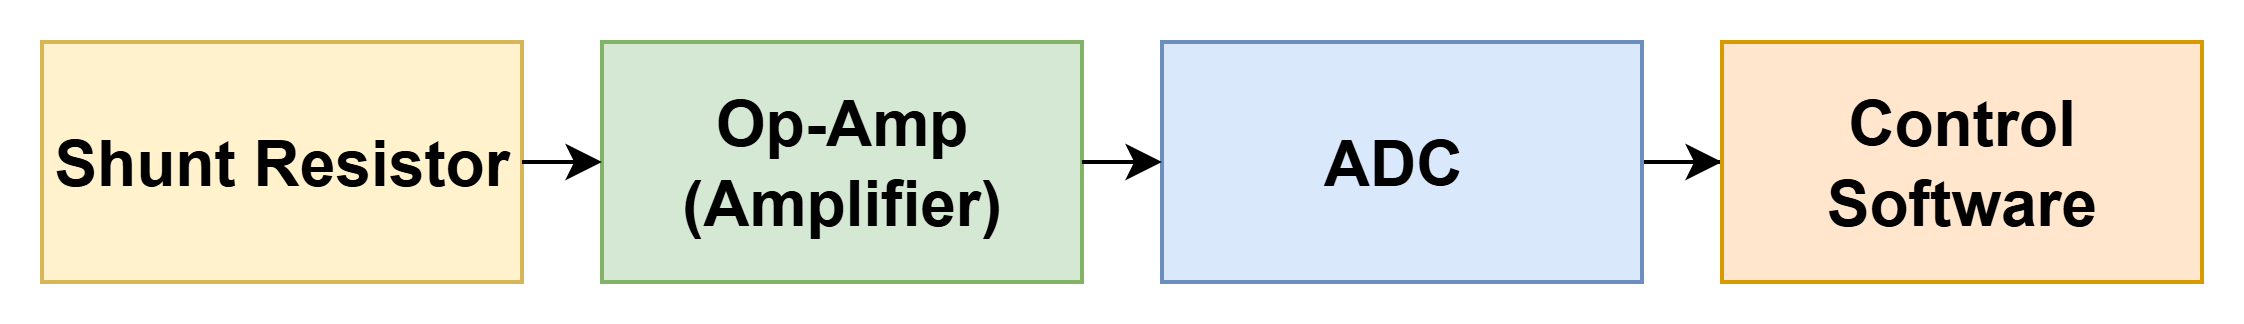
\includegraphics[width=1\linewidth]{signalChain.png}
    \caption{Analogue signal chain, each element adding time delay to the measured signal until the control loop processes}
    \label{fig:controlChain}
\end{figure}

\subsection{Sensorless vs.\ sensored baseline}
In \textbf{sensored} FOC (encoder/resolver), the rotor electrical angle is \emph{measured}, so the alignment error is effectively zero (\(\Delta\theta \approx 0\)). With no angle penalty, the torque expression reduces to

\begin{equation}
T' \;\approx\; \tfrac{3}{2}p\,\lambda\,\big(i_q + e_{i_q}\big),
\end{equation}

so the only path from measurement to torque error is the \emph{current-measurement error} \(e_{i_q}\) itself (plus any inverter ripple), not a compounded \(\cos\Delta\theta\) loss \ref{eq:torque_error}. Practically, this means sensored FOC can tolerate slightly lower current-measurement precision for the same torque ripple/efficiency, because there is no misalignment term multiplying the error \cite{Krishnan2010}.

\medskip
Let \(r \triangleq \epsilon_I / I_{q,\mathrm{rms}}\) be the relative RMS current-measurement error. Copper loss scales with current squared, so:

\begin{equation}
\left.\frac{\Delta P_{\mathrm{cu}}}{P_{\mathrm{cu}}}\right|_{\text{sensored}}
\;\approx\; r^2 .
\end{equation}

In \textbf{sensorless} FOC, current-measurement error \(\epsilon_I\) also drives \emph{angle} error via the estimator sensitivity \(S_{\theta I}\), giving an RMS angle error \(\epsilon_\theta \approx S_{\theta I}\,\epsilon_I\). The misalignment requires extra \(i_q\) by \(1/\cos\Delta\theta\), so from \eqref{eq:cu-loss} the copper-loss increase adds \(\Delta\theta^2\) (small-angle). Hence


\begin{equation}
\left.\frac{\Delta P_{\mathrm{cu}}}{P_{\mathrm{cu}}}\right|_{\text{sensorless}}
\;\approx\; r^2 \;+\; \epsilon_\theta^2
\;=\; r^2 \;+\; \big(S_{\theta I}\,\epsilon_I\big)^2 .
\end{equation}

To map copper-loss growth to \emph{efficiency}, let \(\eta_0\) be the baseline efficiency and \(\kappa\!\triangleq\!P_{\mathrm{cu}}/P_{\mathrm{in}}\) the baseline copper-loss share of input power at the operating point. Holding output power constant,

\begin{equation}
\eta_{\text{sensored}} \;\approx\; \frac{\eta_0}{1+\kappa\,r^2},\qquad
\eta_{\text{sensorless}} \;\approx\; \frac{\eta_0}{1+\kappa\,(r^2+\epsilon_\theta^2)} .
\end{equation}

Thus, even with identical current-measurement quality (\(r\)), sensorless control pays an \emph{extra} efficiency penalty proportional to \(\epsilon_\theta^2\), which is why \(\epsilon_I\) must meet the target from \eqref{eq:I-target} to bound \(\epsilon_\theta\) (and efficiency) \cite{Vas1998,Holtz2002}.


%--------------------------------------------------
% Section 3
%--------------------------------------------------

\section{Sampling Window, Acquisition Time, and Modulation Boundaries}
\label{sec:sampling-window}

With ENOB \emph{assumed adequate} (Sec.~\ref{sec:precision-estimator}), the dominant constraint for accurate current measurement is whether the analog front end can \emph{settle} within the valid sampling window created by the PWM/SVM pattern.

\subsection{Definitions and precondition}
We adopt the precondition from \eqref{eq:precondition}:
\begin{equation}
  \boxed{\, t_{\mathrm{acq}} \;\le\; t_{\mathrm{win}} \,} \qquad
\end{equation}
Here \(t_{\mathrm{acq}}\) is the analog acquisition/settling time to the target error band. \(t_{\mathrm{blank}}\) covers edge-related blanking (deadtime + common-mode/ringing decay), and \(t_{\mathrm{margin}}\) guards against jitter/trigger dispersion. It is convenient to group the requirements for minimum $t_{win}$ as $t_{req}$ required sampling time.
\begin{equation}
  t_{\mathrm{req}} \;\triangleq\; t_{\mathrm{acq}} + t_{\mathrm{blank}} + t_{\mathrm{margin}}.
  \label{eq:treq}
\end{equation}
A sample inside a given active vector is valid if its on-time satisfies \(t_{\mathrm{on}} \ge t_{\mathrm{req}}\). The conversion time \(t_{\mathrm{conv}}\) is \emph{not} rate-limiting provided the sample-and-hold has captured the settled value inside \(t_{\mathrm{win}}\) \cite{Kester2005,Bose2002}.

\begin{figure}
    \centering
    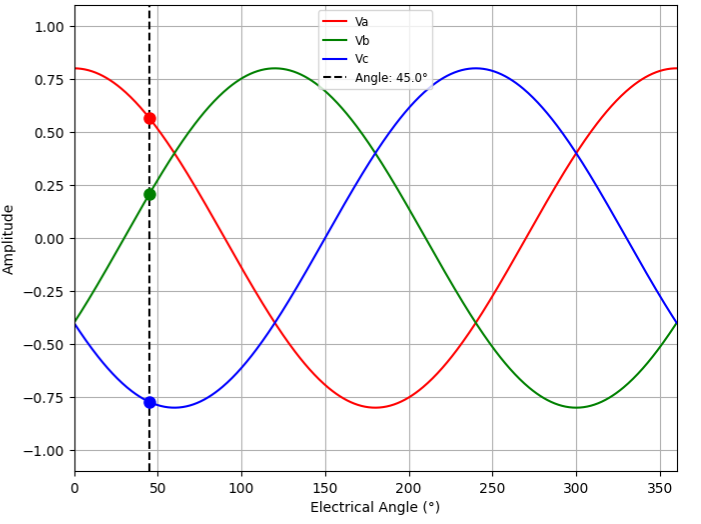
\includegraphics[width=1\linewidth]{Drawings/electricalPosition.png}
    \caption{Electrical position and modulation index ($m=0.80$) defines duty cycles.}
    \label{fig:ElectricalPosition}
\end{figure}

\begin{figure}
    \centering
    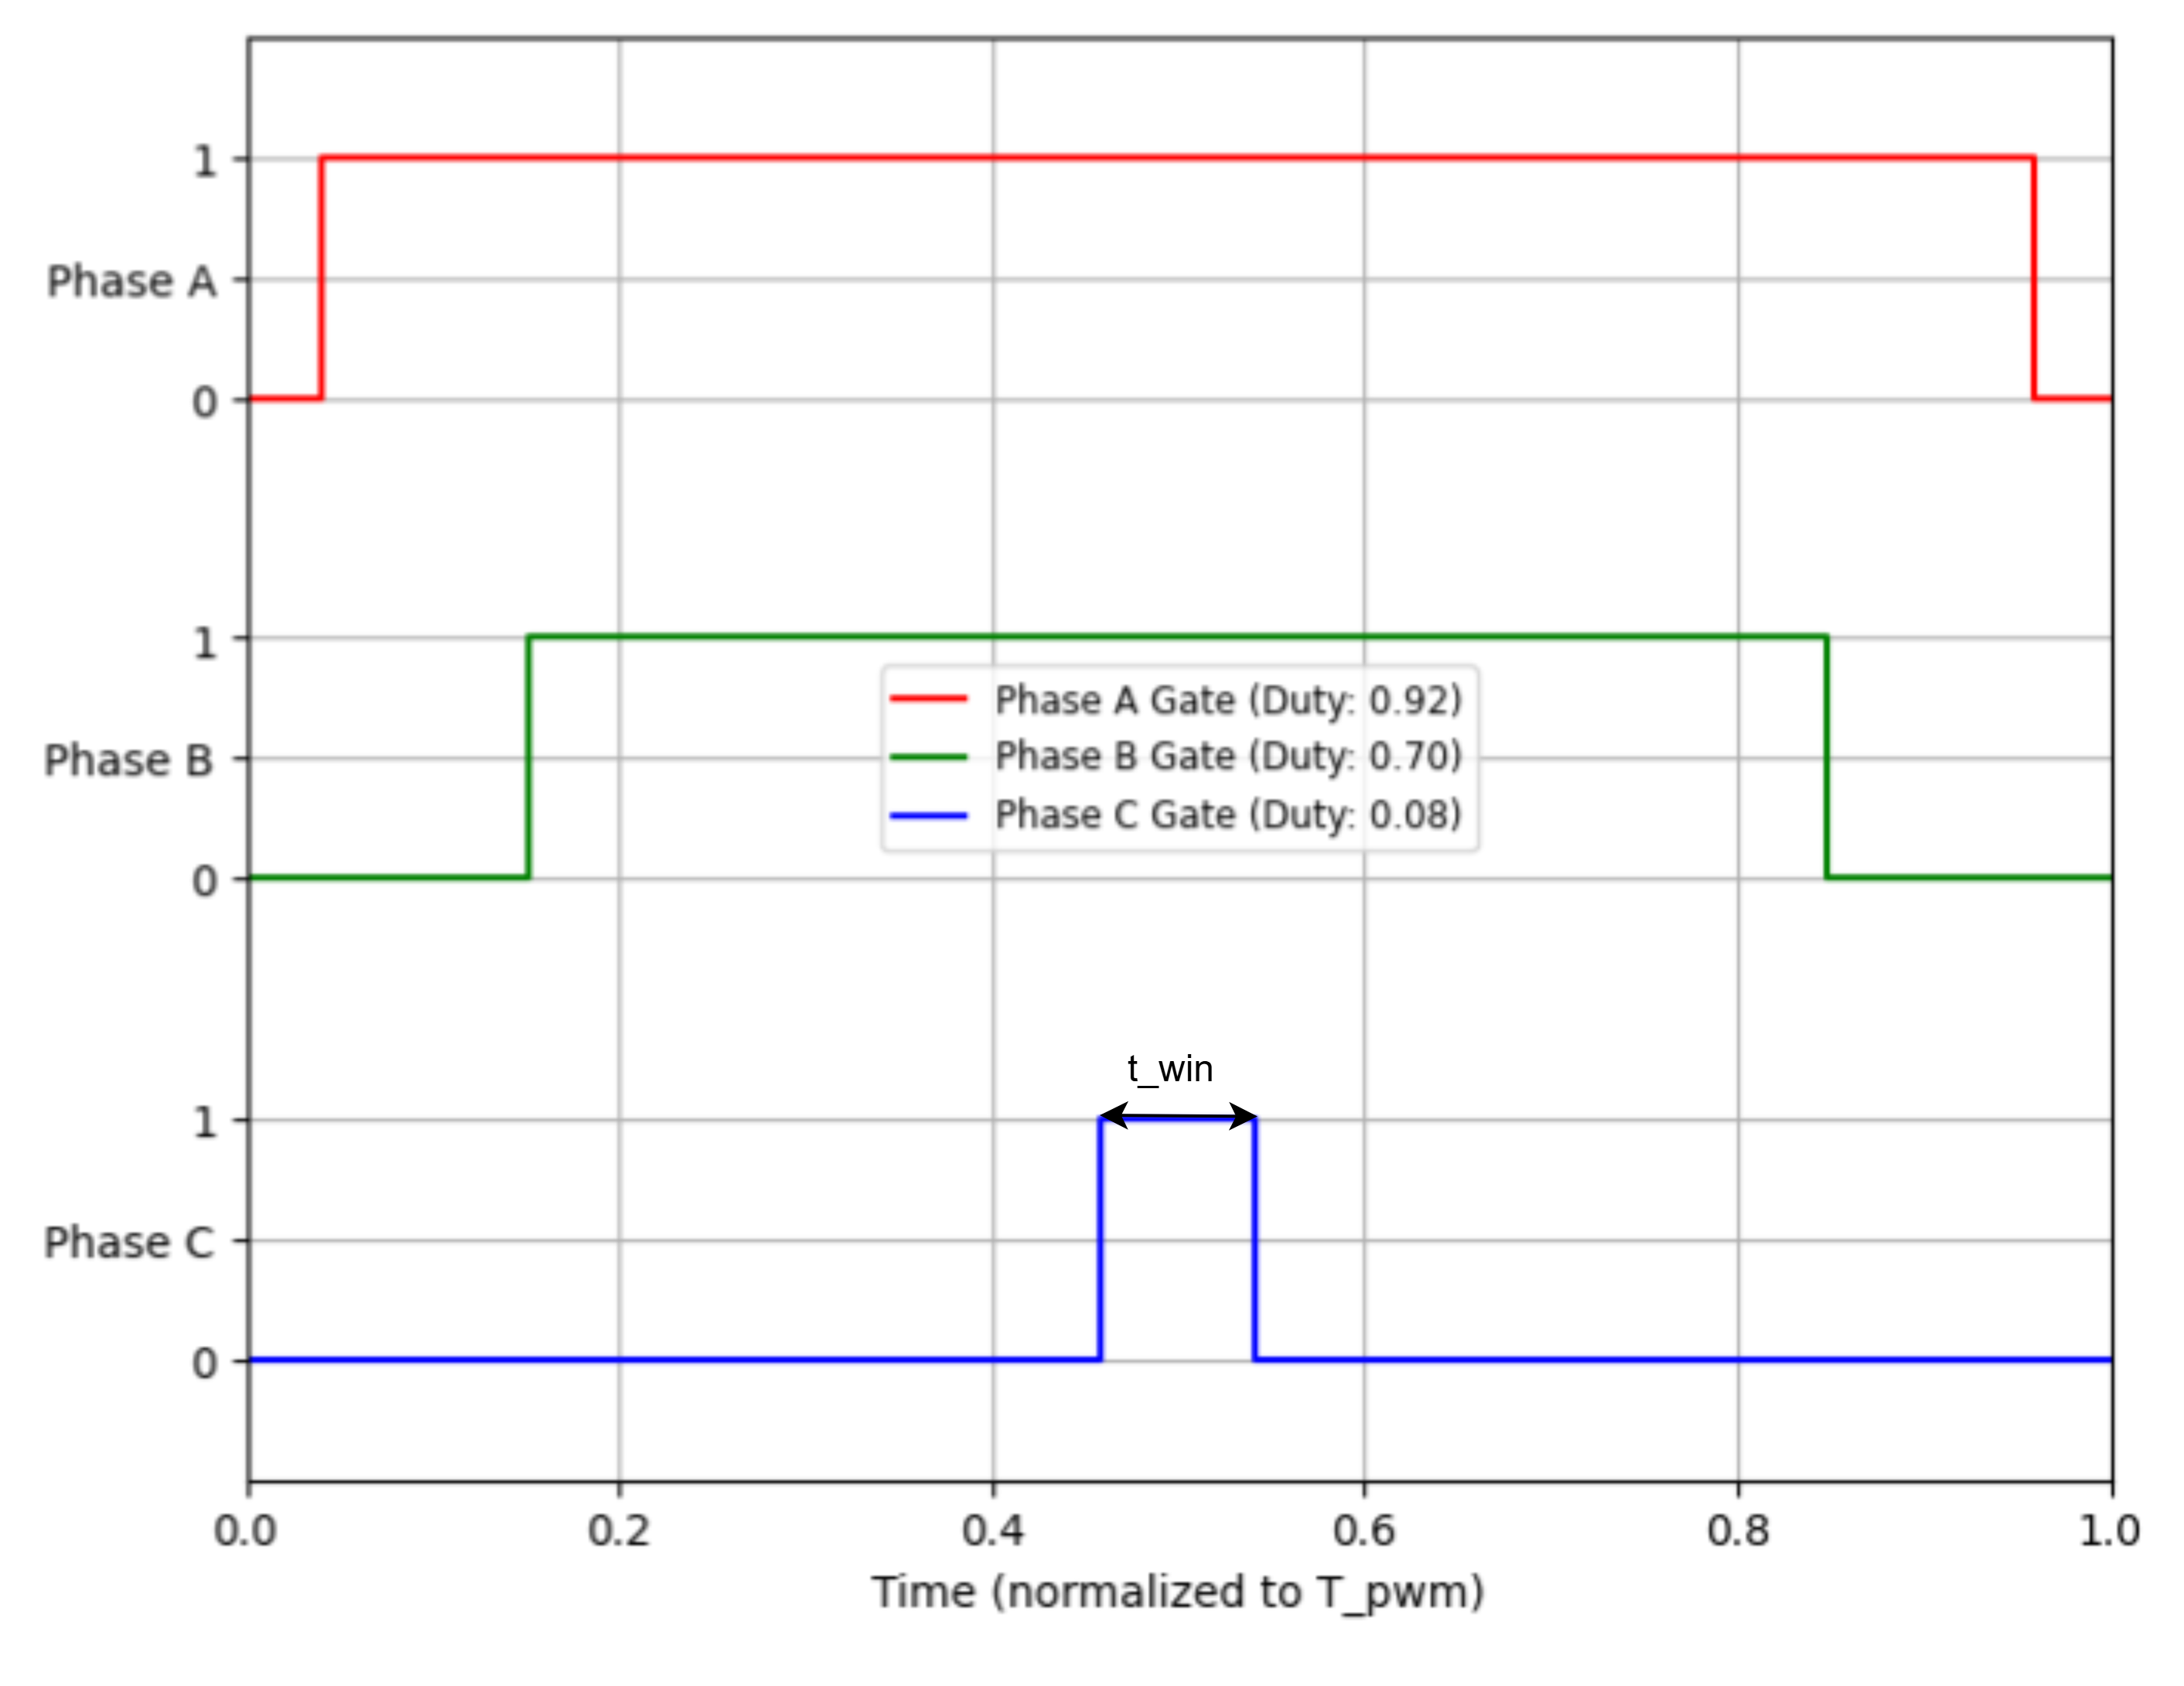
\includegraphics[width=1\linewidth]{Drawings/pwm_mint_window.png}
    \caption{Duty cycle in Phase C is getting to the sampling window limitation ragne.}
    \label{fig:placeholder}
\end{figure}

\subsection{Valid sampling window for dual shunt}
\label{subsec:dual-shunt}
Unlike the single-shunt case, \emph{dual-shunt} sensing does not impose a modulation \emph{lower} bound from settling-time/overlap constraints, because the two phase currents can be sampled at \emph{two distinct instants} within the half-carrier when each measured phase has its own valid plateau. The only hard timing constraint is an \textbf{upper} bound on modulation index \(m\) to keep each measured phase’s plateau long enough to satisfy the required acquisition/settling time \(t_{\mathrm{req}}=t_{\mathrm{acq}}+t_{\mathrm{blank}}+t_{\mathrm{margin}}\).

For center-aligned sinusoidal/SVM modulation, each phase duty is

\begin{equation}
d_a=\tfrac{1}{2}+\tfrac{m}{2}\sin\theta,\quad
\end{equation}
\begin{equation}
d_b=\tfrac{1}{2}+\tfrac{m}{2}\sin(\theta-\tfrac{2\pi}{3}),\quad
\end{equation}
\begin{equation}
d_c=\tfrac{1}{2}+\tfrac{m}{2}\sin(\theta+\tfrac{2\pi}{3}),
\end{equation}

with electrical angle \(\theta\) and modulation index \(m\) as in \eqref{eq:modindex}. A phase’s \emph{shorter} plateau per carrier (low or high, depending on current direction and gating) has length

\begin{equation}
T_{\text{plat},k}^{\min} \;=\; \min\!\big(d_k,\,1-d_k\big)\,T_{sw}
\;\ge\; \Big(\tfrac{1}{2}-\tfrac{m}{2}\Big)T_{sw}\quad
\end{equation}

- worst case over $\theta$ - so guaranteeing a valid sampling window for each measured phase \(k\in\{i,j\}\) requires
\begin{equation}
\Big(\tfrac{1}{2}-\tfrac{m}{2}\Big)T_{sw} \;\ge\; t_{\mathrm{req}}
\;\;\Longrightarrow\;\;
\boxed{~ m \;\le\; 1 - \frac{2\,t_{\mathrm{req}}}{T_{sw}} ~}.
\label{eq:dual-upper}
\end{equation}

\paragraph*{Design takeaway.}
For dual-shunt, settling-time constraints create \emph{no lower bound} on \(m\); the \emph{only} hard bound from \(t_{\mathrm{req}}\) is the \emph{upper} limit \eqref{eq:dual-upper}. Reduce \(t_{\mathrm{acq}}\) (and thus \(t_{\mathrm{req}}\)) to extend usable \(m\) toward 1 without PWM shaping. Otherwise enforce a minimum on-time to guarantee per-phase plateaus at the expense of modulation headroom\cite{ACTAszucs_implementation_2025}.

If a minimum on-time ($t_{\min}$) or clamped SVM is enforced, replace $t_{\mathrm{req}}$ by $\max(t_{\mathrm{req}},t_{\min})$, which tightens the admissible modulation headroom accordingly.


\subsection{Single-shunt sampling window — key challenges}
In single-shunt sensing the valid sampling window exists only within the active-vector plateaus of SVM and \emph{shrinks} near sector edges; two clean samples per half-carrier are required, so losing either window breaks reconstruction. The dominant challenges are \cite{ACTAcabezas_new_2024}:
\begin{itemize}
  \item \textbf{Window dependence on operating point:} Valid windows vary with modulation index and sector angle; “edge” blind zones appear where one dwell time collapses.
  \item \textbf{Acquisition-time budget:} The required time \(t_{\mathrm{req}}=t_{\mathrm{acq}}+t_{\mathrm{blank}}+t_{\mathrm{margin}}\) must fit inside each window; larger \(t_{\mathrm{req}}\) reduces angle coverage and tightens modulation headroom.
  \item \textbf{Trigger determinism \& jitter:} Samples must be placed near vector centers with tight timing; jitter directly converts to current error.
  \item \textbf{PWM shaping trade-offs:} Clamped SVM or enforced minimum on-time can guarantee windows at all angles, but they consume zero-vector dwell and reduce effective voltage (modulation) headroom.
  \item \textbf{Switching-frequency trade-offs:} Lower \(f_{sw}\) enlarges windows but increases current ripple/EMI; higher \(f_{sw}\) does the opposite.
  \item \textbf{Analog front-end realism:} Op-amp/PGA common-mode step response, layout/CMRR, and input RC dominate \(t_{\mathrm{acq}}\). These effects must be validated on hardware, not inferred from MSPS alone.
\end{itemize}
\noindent These challenges govern feasibility once ENOB is adequate; detailed formulas and mitigation strategies (coverage, bounds, and shaping) are deferred to a follow-up paper.



\subsection{Practical example (dual-shunt, 150\,ns ADC + 600\,ns op-amp)}
Assume \(t_{\mathrm{acq}}=0.75~\mu\text{s}\) composed of \textbf{150\,ns} ADC settling and \textbf{600\,ns} op-amp/PGA settling (e.g., DRV8305 at gain 20) \cite{TI_SLAAE96A_2023}. In dual-shunt, settling time imposes \emph{no lower bound} on modulation; the hard constraint is the \emph{upper} bound ensuring each measured phase has a plateau \(\ge t_{\mathrm{req}}=t_{\mathrm{acq}}+t_{\mathrm{blank}}+t_{\mathrm{margin}}\):
\[
\Big(\tfrac{1}{2}-\tfrac{m}{2}\Big)T_{sw} \;\ge\; t_{\mathrm{req}}
\quad\Rightarrow\quad
\boxed{~ m \;\le\; 1 - \frac{2\,t_{\mathrm{req}}}{T_{sw}} ~}.
\]

\paragraph*{Best-case (minimal guard).}
Let \(t_{\mathrm{blank}}{+}t_{\mathrm{margin}}\!\approx\!0 \Rightarrow t_{\mathrm{req}}=0.75~\mu\text{s}\).
At \(f_{sw}=20~\text{kHz}\) (\(T_{sw}=50~\mu\text{s}\)):

\begin{equation}
m_{\max} \;=\; 1 - \frac{2\cdot 0.75}{50} \;\approx\; \mathbf{0.97}.
\end{equation}

Interpretation: you can run essentially up to the linear SVM limit; only the top \(\sim\!3\%\) of modulation is excluded by settling.

\paragraph*{Realistic guard.}
Let \(t_{\mathrm{blank}}{+}t_{\mathrm{margin}}=0.30~\mu\text{s} \Rightarrow t_{\mathrm{req}}=1.05~\mu\text{s}\).
Then

\begin{equation}
m_{\max} \;=\; 1 - \frac{2\cdot 1.05}{50} \;\approx\; \mathbf{0.958}.
\end{equation}

Interpretation: with modest blanking/jitter margin, dual-shunt comfortably supports \(m\!\lesssim\!0.96\) at \(20\) kHz; operation at \(m=0.95\) is fully compatible without PWM shaping.

\begin{equation}
\begin{aligned}
t_{\mathrm{req}}=0.75~\mu\text{s}: \;& d_{\max}=1-\tfrac{0.75}{50}=0.985\;\; d_{\min}=1.5\%.\\
t_{\mathrm{req}}=1.05~\mu\text{s}: \;& d_{\max}=1-\tfrac{1.05}{50}=0.979\;,\;\; d_{\min}=2.1\%.
\end{aligned}
\end{equation}

With the 150\,ns ADC + 600\,ns op-amp settling times, dual-shunt supports per-phase duties up to \(\approx98\%\) (best case) or \(\approx98\%\)–\(97.9\%\) with realistic margins, while maintaining the required settling window on every measured phase.


\subsection*{Section 3 — Summary}
With ENOB already adequate, accurate current sampling hinges on the analog chain settling \emph{inside} the PWM window; define the required window as
\( t_{\mathrm{req}} = t_{\mathrm{acq}} + t_{\mathrm{blank}} + t_{\mathrm{margin}} \),
and note that conversion time is not limiting once the S\&H captures a settled value. For \textbf{dual-shunt}, settling time imposes only an \emph{upper} modulation bound
\( \displaystyle m \le 1 - \frac{2 t_{\mathrm{req}}}{T_{sw}} \),
which also caps the per-phase duty cycle to
\( \displaystyle d_{\max}=1-\frac{t_{\mathrm{req}}}{T_{sw}},\; d_{\min}=\frac{t_{\mathrm{req}}}{T_{sw}} \). The equiation is depending only on PWM frequency and analogue signal chain, but not on ADC bandwith ($t_{conv}$ does not apply). 




% -------------------- Section IV --------------------


\section{Conclusion}
This work reframed dual shunt current sensing for PMSM FOC around \emph{timing geometry}. Once the system ENOB is adequate, maintaining accuracy is dominated by the analog signal chain settles \emph{inside} the PWM/SVM sampling window. The key requirement is the window budget
\(t_{\mathrm{req}} = t_{\mathrm{acq}} + t_{\mathrm{blank}} + t_{\mathrm{margin}}\);
conversion time \(t_{\mathrm{conv}}\) (MSPS) is secondary because the S\&H can convert after a settled capture. 

\medskip
\noindent\textbf{Modulation boundaries from settling time.}
The modulation headroom is set by \(t_{\mathrm{req}}\) and \(T_{sw}\), not by ADC “bandwidth”:
\begin{itemize}
  \item \textbf{Dual-shunt:} no timing-driven \emph{lower} bound on \(m\). The \emph{upper} bound ensuring a valid per-phase plateau is
  \[
     m_{\max} \;=\; 1 - \frac{2 t_{\mathrm{req}}}{T_{sw}}, \qquad
     d_{\max}=1-\frac{t_{\mathrm{req}}}{T_{sw}},\; d_{\min}=\frac{t_{\mathrm{req}}}{T_{sw}}.
  \]
  With the practical chain (150\,ns ADC + 600\,ns op-amp, \(t_{\mathrm{req}}\!\approx\!0.75\text{–}1.05~\mu\)s at 20\,kHz), this supports \(m\!\approx\!0.96\text{–}0.97\) and \(\sim\!98\%\) per-phase duty without PWM shaping.
  \item \textbf{Single-shunt:} Determining the same modulation boundaries equation for single shunt use case is more complex and out of the scope for this paper.
\end{itemize}

\medskip
\noindent\textbf{Impact on efficiency and topology choice.}
Because of current error in sensorless FOC also drives angle error, meeting the timing condition \(t_{\mathrm{acq}}\!\le\!t_{\mathrm{win}}\) directly limits torque misalignment and the associated copper-loss increase. In practice, dual- and three-shunt topologies offer wide windows and simpler timing, while single-shunt remains the most cost- and pin-efficient but is \emph{window-limited} and sensitive to \(t_{\mathrm{req}}\).

\subsection*{Future work}
A companion paper will (i) derive minimum system ENOB targets from application-level \(\epsilon_\theta\) via measured \(S_{\theta I}\), (ii) formalize modulation index boundaries for single-shunt, and (iii) present hardware validation of \(t_{\mathrm{req}}\) under PWM-induced transients.



\bibliographystyle{IEEEtran}
\bibliography{references}

\end{document}


%
1. 
I would like to give a quick overview. Then I want to focus on shunt topologies. Inline, low side 3 phase, low side 2 phase, low side single shunt.
2. 
I want to investigate the precision challange. I want to clarify what precision of current measurement I need to achieve in case of sensorless mode. I want to give a short outlook of sensorless vs sensored measurement and give short comparison that my expectation sensorless FOC needs better current measurement accuracy to reach the same efficiency as the sensored FOC.
3.
My assumption is for ADC requirement is the main driving factor is the position estimator accuracy. The position estimator is impacted by the ADC accuracy. Therefore in the end, impact of the efficiency. Also might be impact on noise. THe main article should be about this part. Additional investigation can be done based on the topology benefits and special requirements. Inline measurement is the easiest regarding the sampling time. Oversample is also possible that increase accuracy. Still there is noise of switching that should be filtered or removed from samples. Or sync the ADC and PWM to not measure in case of switching. Dual shunt and single shunt is aplicable for lower cost applications. But rises the requirements for ADC Aquisition time. I want to highlight that we should talk about acquisition times instead of bandwith. That is much more important than bandwith due to limited sampling window in specific vectors and modulation indexes. In case of writing about modulation index I have to talk about what standard I am using for modulation index. There are blind spots in case of single shunt and also techniques to overcome the challange. But generally if the acqisition time is faster we can stretch the modulation index closer to the boundaries. Also there is consideration of signal chain as external or internal OPAMPS/PGAs has settling time and might limiting the overall acquisituion time. THerefore requires wider sampling window. Again limiting the modulation index boundaries.
4. PWM is not the main part of the article. We may just list basic requirements and good to have features. 
5. I would compare the theoretical as engineering point of view the best is the in line measurement due to the highest accuracy. However in cost, high volume ambedded electronics it is not feasible due to economical limitations, size of the electronics, cost of isolation. Here we may also compare high voltage home appliance >100V and  battery operated requirements <100V. We might bring here some silicon technology limitations due to voltages and integrations. nowadays MCUs is using 22nm that limits opamps/gate driver integrations.
6. Main takeaway should be something like: No cost pressure, Inline measurement is the best and reaches the efficiency of sensored applications. Low cost single shunt is the most cost effective, but minimum xxbit resolution and xbit ENOB accuracy is recommended to keep the control efficiency at x% of sensored control.